\documentclass[a4paper]{book}
\usepackage{a4wide}
\usepackage{makeidx}
\usepackage{fancyhdr}
\usepackage{graphicx}
\usepackage{multicol}
\usepackage{float}
\usepackage{textcomp}
\usepackage{alltt}
\usepackage{times}
\usepackage{ifpdf}
\ifpdf
\usepackage[pdftex,
            pagebackref=true,
            colorlinks=true,
            linkcolor=blue,
            unicode
           ]{hyperref}
\else
\usepackage[ps2pdf,
            pagebackref=true,
            colorlinks=true,
            linkcolor=blue,
            unicode
           ]{hyperref}
\usepackage{pspicture}
\fi
\usepackage[utf8]{inputenc}
\usepackage{doxygen}
\makeindex
\setcounter{tocdepth}{3}
\renewcommand{\footrulewidth}{0.4pt}
\begin{document}
\begin{titlepage}
\vspace*{7cm}
\begin{center}
{\Large TangoInterface }\\
\vspace*{1cm}
{\large Generated by Doxygen 1.5.6}\\
\vspace*{0.5cm}
{\small Fri Dec 4 12:49:14 2009}\\
\end{center}
\end{titlepage}
\clearemptydoublepage
\pagenumbering{roman}
\tableofcontents
\clearemptydoublepage
\pagenumbering{arabic}
\chapter{Class Index}
\section{Class List}
Here are the classes, structs, unions and interfaces with brief descriptions:\begin{CompactList}
\item\contentsline{section}{\hyperlink{classCTangoInterfaceApp}{CTangoInterfaceApp} }{\pageref{classCTangoInterfaceApp}}{}
\item\contentsline{section}{\hyperlink{classTangoInterface}{TangoInterface} }{\pageref{classTangoInterface}}{}
\end{CompactList}

\chapter{File Index}
\section{File List}
Here is a list of all files with brief descriptions:\begin{CompactList}
\item\contentsline{section}{/homenfs/amilan/workspace/Xradia-dll/LastVersion/TangoInterface\_\-20091201/\hyperlink{Resource_8h}{Resource.h} }{\pageref{Resource_8h}}{}
\item\contentsline{section}{/homenfs/amilan/workspace/Xradia-dll/LastVersion/TangoInterface\_\-20091201/\hyperlink{stdafx_8cpp}{stdafx.cpp} }{\pageref{stdafx_8cpp}}{}
\item\contentsline{section}{/homenfs/amilan/workspace/Xradia-dll/LastVersion/TangoInterface\_\-20091201/\hyperlink{stdafx_8h}{stdafx.h} }{\pageref{stdafx_8h}}{}
\item\contentsline{section}{/homenfs/amilan/workspace/Xradia-dll/LastVersion/TangoInterface\_\-20091201/\hyperlink{TangoInterface_8cpp}{TangoInterface.cpp} }{\pageref{TangoInterface_8cpp}}{}
\item\contentsline{section}{/homenfs/amilan/workspace/Xradia-dll/LastVersion/TangoInterface\_\-20091201/\hyperlink{TangoInterface_8h}{TangoInterface.h} }{\pageref{TangoInterface_8h}}{}
\item\contentsline{section}{/homenfs/amilan/workspace/Xradia-dll/LastVersion/TangoInterface\_\-20091201/\hyperlink{TangoInterfaceApp_8cpp}{TangoInterfaceApp.cpp} }{\pageref{TangoInterfaceApp_8cpp}}{}
\item\contentsline{section}{/homenfs/amilan/workspace/Xradia-dll/LastVersion/TangoInterface\_\-20091201/\hyperlink{TangoInterfaceApp_8h}{TangoInterfaceApp.h} }{\pageref{TangoInterfaceApp_8h}}{}
\item\contentsline{section}{/homenfs/amilan/workspace/Xradia-dll/LastVersion/TangoInterface\_\-20091201/\hyperlink{targetver_8h}{targetver.h} }{\pageref{targetver_8h}}{}
\end{CompactList}

\chapter{Class Documentation}
\hypertarget{classCTangoInterfaceApp}{
\section{CTangoInterfaceApp Class Reference}
\label{classCTangoInterfaceApp}\index{CTangoInterfaceApp@{CTangoInterfaceApp}}
}
{\tt \#include $<$TangoInterfaceApp.h$>$}

\subsection*{Public Member Functions}
\begin{CompactItemize}
\item 
\hyperlink{classCTangoInterfaceApp_e1aaadbba6f66b517068a5ec68ea344e}{CTangoInterfaceApp} ()
\item 
virtual BOOL \hyperlink{classCTangoInterfaceApp_1e4456db86ea4dfa641d244a7715b4f6}{InitInstance} ()
\end{CompactItemize}


\subsection{Constructor \& Destructor Documentation}
\hypertarget{classCTangoInterfaceApp_e1aaadbba6f66b517068a5ec68ea344e}{
\index{CTangoInterfaceApp@{CTangoInterfaceApp}!CTangoInterfaceApp@{CTangoInterfaceApp}}
\index{CTangoInterfaceApp@{CTangoInterfaceApp}!CTangoInterfaceApp@{CTangoInterfaceApp}}
\subsubsection[CTangoInterfaceApp]{\setlength{\rightskip}{0pt plus 5cm}CTangoInterfaceApp::CTangoInterfaceApp ()}}
\label{classCTangoInterfaceApp_e1aaadbba6f66b517068a5ec68ea344e}




\subsection{Member Function Documentation}
\hypertarget{classCTangoInterfaceApp_1e4456db86ea4dfa641d244a7715b4f6}{
\index{CTangoInterfaceApp@{CTangoInterfaceApp}!InitInstance@{InitInstance}}
\index{InitInstance@{InitInstance}!CTangoInterfaceApp@{CTangoInterfaceApp}}
\subsubsection[InitInstance]{\setlength{\rightskip}{0pt plus 5cm}BOOL CTangoInterfaceApp::InitInstance ()\hspace{0.3cm}{\tt  \mbox{[}virtual\mbox{]}}}}
\label{classCTangoInterfaceApp_1e4456db86ea4dfa641d244a7715b4f6}




The documentation for this class was generated from the following files:\begin{CompactItemize}
\item 
/homenfs/amilan/workspace/Xradia-dll/LastVersion/TangoInterface\_\-20091201/\hyperlink{TangoInterfaceApp_8h}{TangoInterfaceApp.h}\item 
/homenfs/amilan/workspace/Xradia-dll/LastVersion/TangoInterface\_\-20091201/\hyperlink{TangoInterfaceApp_8cpp}{TangoInterfaceApp.cpp}\end{CompactItemize}

\hypertarget{classTangoInterface}{
\section{TangoInterface Class Reference}
\label{classTangoInterface}\index{TangoInterface@{TangoInterface}}
}
{\tt \#include $<$TangoInterface.h$>$}

\subsection*{Public Member Functions}
\begin{CompactItemize}
\item 
\hyperlink{classTangoInterface_075eeb694387d0a1621cfdcfe06d222f}{TangoInterface} (void)
\begin{CompactList}\small\item\em Default constructor. \item\end{CompactList}\item 
\hyperlink{classTangoInterface_6af2d055005412be8ad30be0eada083b}{$\sim$TangoInterface} (void)
\begin{CompactList}\small\item\em Destructor. \item\end{CompactList}\item 
bool \hyperlink{classTangoInterface_e4c5af1c2055bdd253eddce0babd9158}{GetErrorMessage} (CString \&strErrorMsg)
\begin{CompactList}\small\item\em Gets an error message. \item\end{CompactList}\item 
bool \hyperlink{classTangoInterface_45f902f0d486ff896b49de74d2e60a02}{SetMotorSpeed} (CString strMotorIdentifier, float fSpeed)
\begin{CompactList}\small\item\em Sets the motor speed. \item\end{CompactList}\item 
bool \hyperlink{classTangoInterface_c14b1a6b2d195d30a26b02fdffd81428}{GetMotorPosition} (CString strMotorIdentifier, float \&fPosition)
\begin{CompactList}\small\item\em Gets the motor position. \item\end{CompactList}\item 
bool \hyperlink{classTangoInterface_e7b82506f5a1c901fd7f5e0843841c7d}{EnableMotor} (CString strMotorIdentifier, bool bEnable)
\begin{CompactList}\small\item\em Enables the motor. \item\end{CompactList}\item 
bool \hyperlink{classTangoInterface_ab781c1b152882cff163edd81407033f}{JogMotor} (CString strMotorIdentifier, bool bMovePositive)
\begin{CompactList}\small\item\em Jog motor. \item\end{CompactList}\item 
bool \hyperlink{classTangoInterface_98190a21946b4aa04b7d4b12ababa768}{GetHomingStatus} (CString strMotorIdentifier, int \&nHomingStatus)
\begin{CompactList}\small\item\em Get the homing status. \item\end{CompactList}\item 
bool \hyperlink{classTangoInterface_e6da63765a09f8c53a8537faee7f63b5}{Home} (CString strMotorIdentifier)
\begin{CompactList}\small\item\em Issues the Home command. \item\end{CompactList}\item 
bool \hyperlink{classTangoInterface_9db5a121d918ac94527d5e3fc635d002}{MoveMotor} (CString strMotorIdentifier, float fPosition)
\begin{CompactList}\small\item\em Move motor. \item\end{CompactList}\item 
bool \hyperlink{classTangoInterface_c37a6c8ebf341566b1cba2ce56630811}{SetVariable} (CString strVariableName, CString strValue)
\begin{CompactList}\small\item\em Sets a variable. \item\end{CompactList}\item 
bool \hyperlink{classTangoInterface_ded717121a0c221a3b7528d221d24657}{SetVariable} (CString strVariableName, int nValue)
\begin{CompactList}\small\item\em Sets a variable. \item\end{CompactList}\item 
bool \hyperlink{classTangoInterface_bbad345c34f9c25f013be3bbc02cfe96}{SetVariable} (CString strVariableName, float fValue)
\begin{CompactList}\small\item\em Sets a variable. \item\end{CompactList}\item 
bool \hyperlink{classTangoInterface_d99eec46ef2205c72d4dc562154f6474}{SetVariable} (CString strVariableName, bool bValue)
\begin{CompactList}\small\item\em Sets a variable. \item\end{CompactList}\item 
bool \hyperlink{classTangoInterface_f981459258550748b98541a18c6e8f54}{GetVariableFloat} (CString strVariableName, float \&fValue)
\begin{CompactList}\small\item\em Gets a variable (float version). \item\end{CompactList}\item 
bool \hyperlink{classTangoInterface_ea841d48dfb2d66019268beda8ba2da5}{GetVariableInt} (CString strVariableName, int \&nValue)
\begin{CompactList}\small\item\em Gets a variable (integer version). \item\end{CompactList}\item 
bool \hyperlink{classTangoInterface_90bceaea83a14b34d3a6c4dca7f5756b}{GetVariableString} (CString strVariableName, CString \&strReturn)
\begin{CompactList}\small\item\em Gets a variable (string version). \item\end{CompactList}\item 
bool \hyperlink{classTangoInterface_92743acefced68c408d846813dba4697}{GetVariableBool} (CString strVariableName, bool \&bValue)
\begin{CompactList}\small\item\em Gets a variable (boolean version). \item\end{CompactList}\item 
bool \hyperlink{classTangoInterface_c2f7cbbe72be043cbadf73a8bf23654d}{GetMotorVariableFloat} (CString strMotorIdentifier, CString strVariableName, float \&fValue)
\begin{CompactList}\small\item\em Get a motor variable (float version). \item\end{CompactList}\item 
bool \hyperlink{classTangoInterface_22a22602be1fef00ab7376be40b58ff4}{GetMotorVariableInt} (CString strMotorIdentifier, CString strVariableName, int \&nValue)
\begin{CompactList}\small\item\em Get a motor variable (integer version). \item\end{CompactList}\item 
bool \hyperlink{classTangoInterface_2d5610cce92ea977ad74202219b1a0af}{GetMotorVariableString} (CString strMotorIdentifier, CString strVariableName, CString \&strReturn)
\begin{CompactList}\small\item\em Get a motor variable (string version). \item\end{CompactList}\item 
bool \hyperlink{classTangoInterface_8b0eb830867b7d62dc4350b49b430705}{GetMotorVariableBool} (CString strMotorIdentifier, CString strVariableName, bool \&bValue)
\begin{CompactList}\small\item\em Get a motor variable (boolean version). \item\end{CompactList}\item 
int \hyperlink{classTangoInterface_78ab845a344c3d140cbeef3da653ca29}{GetMotorAttributeStrings} (CString $\ast$\&pstrVariableNames, int nNumAttributes)
\begin{CompactList}\small\item\em Gets a specified list of motor variable names. \item\end{CompactList}\end{CompactItemize}


\subsection{Constructor \& Destructor Documentation}
\hypertarget{classTangoInterface_075eeb694387d0a1621cfdcfe06d222f}{
\index{TangoInterface@{TangoInterface}!TangoInterface@{TangoInterface}}
\index{TangoInterface@{TangoInterface}!TangoInterface@{TangoInterface}}
\subsubsection[TangoInterface]{\setlength{\rightskip}{0pt plus 5cm}TangoInterface::TangoInterface (void)}}
\label{classTangoInterface_075eeb694387d0a1621cfdcfe06d222f}


Default constructor. 

\hypertarget{classTangoInterface_6af2d055005412be8ad30be0eada083b}{
\index{TangoInterface@{TangoInterface}!$\sim$TangoInterface@{$\sim$TangoInterface}}
\index{$\sim$TangoInterface@{$\sim$TangoInterface}!TangoInterface@{TangoInterface}}
\subsubsection[$\sim$TangoInterface]{\setlength{\rightskip}{0pt plus 5cm}TangoInterface::$\sim$TangoInterface (void)}}
\label{classTangoInterface_6af2d055005412be8ad30be0eada083b}


Destructor. 



\subsection{Member Function Documentation}
\hypertarget{classTangoInterface_e4c5af1c2055bdd253eddce0babd9158}{
\index{TangoInterface@{TangoInterface}!GetErrorMessage@{GetErrorMessage}}
\index{GetErrorMessage@{GetErrorMessage}!TangoInterface@{TangoInterface}}
\subsubsection[GetErrorMessage]{\setlength{\rightskip}{0pt plus 5cm}bool TangoInterface::GetErrorMessage (CString \& {\em strErrorMsg})}}
\label{classTangoInterface_e4c5af1c2055bdd253eddce0babd9158}


Gets an error message. 

Will return an error string describing the most recent failure.

\begin{Desc}
\item[Parameters:]
\begin{description}
\item[{\em strErrorMsg}]CString to recieve the error message string. \end{description}
\end{Desc}


\begin{Desc}
\item[Returns:]true if the command succeeds, false if the command fails. \end{Desc}
\hypertarget{classTangoInterface_45f902f0d486ff896b49de74d2e60a02}{
\index{TangoInterface@{TangoInterface}!SetMotorSpeed@{SetMotorSpeed}}
\index{SetMotorSpeed@{SetMotorSpeed}!TangoInterface@{TangoInterface}}
\subsubsection[SetMotorSpeed]{\setlength{\rightskip}{0pt plus 5cm}bool TangoInterface::SetMotorSpeed (CString {\em strMotorIdentifier}, \/  float {\em fSpeed})}}
\label{classTangoInterface_45f902f0d486ff896b49de74d2e60a02}


Sets the motor speed. 

\begin{Desc}
\item[Parameters:]
\begin{description}
\item[{\em strMotorIdentifier}]The motor identifier for the motor of interest.\item[{\em fSpeed}]The speed value to set in counts per second. \end{description}
\end{Desc}


\begin{Desc}
\item[Returns:]true if the command succeeds, false if the command fails. \end{Desc}
\hypertarget{classTangoInterface_c14b1a6b2d195d30a26b02fdffd81428}{
\index{TangoInterface@{TangoInterface}!GetMotorPosition@{GetMotorPosition}}
\index{GetMotorPosition@{GetMotorPosition}!TangoInterface@{TangoInterface}}
\subsubsection[GetMotorPosition]{\setlength{\rightskip}{0pt plus 5cm}bool TangoInterface::GetMotorPosition (CString {\em strMotorIdentifier}, \/  float \& {\em fPosition})}}
\label{classTangoInterface_c14b1a6b2d195d30a26b02fdffd81428}


Gets the motor position. 

\begin{Desc}
\item[Parameters:]
\begin{description}
\item[{\em strMotorIdentifier}]The motor identifier for the motor of interest.\item[{\em fPosition}]The motor position in counts. \end{description}
\end{Desc}


\begin{Desc}
\item[Returns:]true if the command succeeds, false if the command fails. \end{Desc}
\hypertarget{classTangoInterface_e7b82506f5a1c901fd7f5e0843841c7d}{
\index{TangoInterface@{TangoInterface}!EnableMotor@{EnableMotor}}
\index{EnableMotor@{EnableMotor}!TangoInterface@{TangoInterface}}
\subsubsection[EnableMotor]{\setlength{\rightskip}{0pt plus 5cm}bool TangoInterface::EnableMotor (CString {\em strMotorIdentifier}, \/  bool {\em bEnable})}}
\label{classTangoInterface_e7b82506f5a1c901fd7f5e0843841c7d}


Enables the motor. 

\begin{Desc}
\item[Parameters:]
\begin{description}
\item[{\em strMotorIdentifier}]The motor identifier for the motor of interest.\item[{\em bEnable}]true to enable it, false to disable it. \end{description}
\end{Desc}


\begin{Desc}
\item[Returns:]true if the command succeeds, false if the command fails. \end{Desc}
\hypertarget{classTangoInterface_ab781c1b152882cff163edd81407033f}{
\index{TangoInterface@{TangoInterface}!JogMotor@{JogMotor}}
\index{JogMotor@{JogMotor}!TangoInterface@{TangoInterface}}
\subsubsection[JogMotor]{\setlength{\rightskip}{0pt plus 5cm}bool TangoInterface::JogMotor (CString {\em strMotorIdentifier}, \/  bool {\em bMovePositive})}}
\label{classTangoInterface_ab781c1b152882cff163edd81407033f}


Jog motor. 

This will cause the motor of interest to jog continuously in the specified direction.

\begin{Desc}
\item[Parameters:]
\begin{description}
\item[{\em strMotorIdentifier}]The motor identifier for the motor of interest.\item[{\em bMovePositive}]Direction to Jog. True for Positive, False for negative. \end{description}
\end{Desc}


\begin{Desc}
\item[Returns:]true if the command succeeds, false if the command fails. \end{Desc}
\hypertarget{classTangoInterface_98190a21946b4aa04b7d4b12ababa768}{
\index{TangoInterface@{TangoInterface}!GetHomingStatus@{GetHomingStatus}}
\index{GetHomingStatus@{GetHomingStatus}!TangoInterface@{TangoInterface}}
\subsubsection[GetHomingStatus]{\setlength{\rightskip}{0pt plus 5cm}bool TangoInterface::GetHomingStatus (CString {\em strMotorIdentifier}, \/  int \& {\em nHomingStatus})}}
\label{classTangoInterface_98190a21946b4aa04b7d4b12ababa768}


Get the homing status. 

Minimum necessary implemenation requires this function to return values 0 and 15. These corresponds to \char`\"{}homing not started\char`\"{} and \char`\"{}homing complete\char`\"{}. If the motor does not require or allow homing this function, this function should return 15, home complete. /remarks$>$ \begin{Desc}
\item[Parameters:]
\begin{description}
\item[{\em strMotorIdentifier}]The motor identifier for the motor of interest.\item[{\em nHomingStatus}]The homing status defined by the values 0-17 with the following definitions: HomingRoutineNotStartedYet = 0, WaitingforOther = 1, MovingToLimit = 2, IsAtLimit = 3, MovingToCoarseHome = 4, MovingToFixedOffset = 5, MovingToFineHome = 6, IsAtHome = 7, MovingToAlignedPos = 8, FollowedoutOnCoarse = 9, FollowedoutOnFixedOffset = 10, FollowedoutOnFineHome = 11, FollowedoutOnAlignedPos = 12, HitLimitOnFineHome = 13, HitLimitOnAlignedPos = 14, HomeComplete = 15, GeneralError = 16, PreconditionNotMet = 17 \end{description}
\end{Desc}


\begin{Desc}
\item[Returns:]true if the command succeeds, false if the command fails. \end{Desc}
\hypertarget{classTangoInterface_e6da63765a09f8c53a8537faee7f63b5}{
\index{TangoInterface@{TangoInterface}!Home@{Home}}
\index{Home@{Home}!TangoInterface@{TangoInterface}}
\subsubsection[Home]{\setlength{\rightskip}{0pt plus 5cm}bool TangoInterface::Home (CString {\em strMotorIdentifier})}}
\label{classTangoInterface_e6da63765a09f8c53a8537faee7f63b5}


Issues the Home command. 

This command will cause the specified motor to initiate the homing process. If the motor does not require or allow homing this function, this function should return true.

\begin{Desc}
\item[Parameters:]
\begin{description}
\item[{\em strMotorIdentifier}]The motor identifier for the motor of interest.\end{description}
\end{Desc}


\begin{Desc}
\item[Returns:]true if the command succeeds, false if the command fails. \end{Desc}
\hypertarget{classTangoInterface_9db5a121d918ac94527d5e3fc635d002}{
\index{TangoInterface@{TangoInterface}!MoveMotor@{MoveMotor}}
\index{MoveMotor@{MoveMotor}!TangoInterface@{TangoInterface}}
\subsubsection[MoveMotor]{\setlength{\rightskip}{0pt plus 5cm}bool TangoInterface::MoveMotor (CString {\em strMotorIdentifier}, \/  float {\em fPosition})}}
\label{classTangoInterface_9db5a121d918ac94527d5e3fc635d002}


Move motor. 

\begin{Desc}
\item[Parameters:]
\begin{description}
\item[{\em strMotorIdentifier}]The motor identifier for the motor of interest.\item[{\em fPosition}]The ABSOLUTE position in counts. \end{description}
\end{Desc}


\begin{Desc}
\item[Returns:]true if the command succeeds, false if the command fails. \end{Desc}
\hypertarget{classTangoInterface_c37a6c8ebf341566b1cba2ce56630811}{
\index{TangoInterface@{TangoInterface}!SetVariable@{SetVariable}}
\index{SetVariable@{SetVariable}!TangoInterface@{TangoInterface}}
\subsubsection[SetVariable]{\setlength{\rightskip}{0pt plus 5cm}bool TangoInterface::SetVariable (CString {\em strVariableName}, \/  CString {\em strValue})}}
\label{classTangoInterface_c37a6c8ebf341566b1cba2ce56630811}


Sets a variable. 

Sets the specified variable to the specified value.

\begin{Desc}
\item[Parameters:]
\begin{description}
\item[{\em strVariableName}]The variable name. \item[{\em strValue}]The value as a string. \end{description}
\end{Desc}


\begin{Desc}
\item[Returns:]true if the command succeeds, false if the command fails. \end{Desc}
\hypertarget{classTangoInterface_ded717121a0c221a3b7528d221d24657}{
\index{TangoInterface@{TangoInterface}!SetVariable@{SetVariable}}
\index{SetVariable@{SetVariable}!TangoInterface@{TangoInterface}}
\subsubsection[SetVariable]{\setlength{\rightskip}{0pt plus 5cm}bool TangoInterface::SetVariable (CString {\em strVariableName}, \/  int {\em nValue})}}
\label{classTangoInterface_ded717121a0c221a3b7528d221d24657}


Sets a variable. 

Sets the specified variable to the specified value.

\begin{Desc}
\item[Parameters:]
\begin{description}
\item[{\em strVariableName}]The variable name. \item[{\em strValue}]The value as an integer. \end{description}
\end{Desc}


\begin{Desc}
\item[Returns:]true if the command succeeds, false if the command fails. \end{Desc}
\hypertarget{classTangoInterface_bbad345c34f9c25f013be3bbc02cfe96}{
\index{TangoInterface@{TangoInterface}!SetVariable@{SetVariable}}
\index{SetVariable@{SetVariable}!TangoInterface@{TangoInterface}}
\subsubsection[SetVariable]{\setlength{\rightskip}{0pt plus 5cm}bool TangoInterface::SetVariable (CString {\em strVariableName}, \/  float {\em fValue})}}
\label{classTangoInterface_bbad345c34f9c25f013be3bbc02cfe96}


Sets a variable. 

Sets the specified variable to the specified value.

\begin{Desc}
\item[Parameters:]
\begin{description}
\item[{\em strVariableName}]The variable name. \item[{\em strValue}]The value as a float. \end{description}
\end{Desc}


\begin{Desc}
\item[Returns:]true if the command succeeds, false if the command fails. \end{Desc}
\hypertarget{classTangoInterface_d99eec46ef2205c72d4dc562154f6474}{
\index{TangoInterface@{TangoInterface}!SetVariable@{SetVariable}}
\index{SetVariable@{SetVariable}!TangoInterface@{TangoInterface}}
\subsubsection[SetVariable]{\setlength{\rightskip}{0pt plus 5cm}bool TangoInterface::SetVariable (CString {\em strVariableName}, \/  bool {\em bValue})}}
\label{classTangoInterface_d99eec46ef2205c72d4dc562154f6474}


Sets a variable. 

Sets the specified variable to the specified value.

\begin{Desc}
\item[Parameters:]
\begin{description}
\item[{\em strVariableName}]The variable name. \item[{\em strValue}]The value as a boolean. \end{description}
\end{Desc}


\begin{Desc}
\item[Returns:]true if the command succeeds, false if the command fails. \end{Desc}
\hypertarget{classTangoInterface_f981459258550748b98541a18c6e8f54}{
\index{TangoInterface@{TangoInterface}!GetVariableFloat@{GetVariableFloat}}
\index{GetVariableFloat@{GetVariableFloat}!TangoInterface@{TangoInterface}}
\subsubsection[GetVariableFloat]{\setlength{\rightskip}{0pt plus 5cm}bool TangoInterface::GetVariableFloat (CString {\em strVariableName}, \/  float \& {\em fValue})}}
\label{classTangoInterface_f981459258550748b98541a18c6e8f54}


Gets a variable (float version). 

Gets the value of the specified variable.

\begin{Desc}
\item[Parameters:]
\begin{description}
\item[{\em strVariableName}]The variable name. \item[{\em fValue}]the variable value. \end{description}
\end{Desc}


\begin{Desc}
\item[Returns:]true if the command succeeds, false if the command fails. \end{Desc}
\hypertarget{classTangoInterface_ea841d48dfb2d66019268beda8ba2da5}{
\index{TangoInterface@{TangoInterface}!GetVariableInt@{GetVariableInt}}
\index{GetVariableInt@{GetVariableInt}!TangoInterface@{TangoInterface}}
\subsubsection[GetVariableInt]{\setlength{\rightskip}{0pt plus 5cm}bool TangoInterface::GetVariableInt (CString {\em strVariableName}, \/  int \& {\em nValue})}}
\label{classTangoInterface_ea841d48dfb2d66019268beda8ba2da5}


Gets a variable (integer version). 

Gets the value of the specified variable.

\begin{Desc}
\item[Parameters:]
\begin{description}
\item[{\em strVariableName}]The variable name. \item[{\em nValue}]the variable value. \end{description}
\end{Desc}


\begin{Desc}
\item[Returns:]true if the command succeeds, false if the command fails. \end{Desc}
\hypertarget{classTangoInterface_90bceaea83a14b34d3a6c4dca7f5756b}{
\index{TangoInterface@{TangoInterface}!GetVariableString@{GetVariableString}}
\index{GetVariableString@{GetVariableString}!TangoInterface@{TangoInterface}}
\subsubsection[GetVariableString]{\setlength{\rightskip}{0pt plus 5cm}bool TangoInterface::GetVariableString (CString {\em strVariableName}, \/  CString \& {\em strReturn})}}
\label{classTangoInterface_90bceaea83a14b34d3a6c4dca7f5756b}


Gets a variable (string version). 

Gets the value of the specified variable.

\begin{Desc}
\item[Parameters:]
\begin{description}
\item[{\em strVariableName}]The variable name. \item[{\em strReturn}]The variable value. \end{description}
\end{Desc}


\begin{Desc}
\item[Returns:]true if the command succeeds, false if the command fails. \end{Desc}
\hypertarget{classTangoInterface_92743acefced68c408d846813dba4697}{
\index{TangoInterface@{TangoInterface}!GetVariableBool@{GetVariableBool}}
\index{GetVariableBool@{GetVariableBool}!TangoInterface@{TangoInterface}}
\subsubsection[GetVariableBool]{\setlength{\rightskip}{0pt plus 5cm}bool TangoInterface::GetVariableBool (CString {\em strVariableName}, \/  bool \& {\em bValue})}}
\label{classTangoInterface_92743acefced68c408d846813dba4697}


Gets a variable (boolean version). 

Gets the value of the specified variable.

\begin{Desc}
\item[Parameters:]
\begin{description}
\item[{\em strVariableName}]The variable name. \item[{\em bValue}]The variable value. \end{description}
\end{Desc}


\begin{Desc}
\item[Returns:]true if the command succeeds, false if the command fails. \end{Desc}
\hypertarget{classTangoInterface_c2f7cbbe72be043cbadf73a8bf23654d}{
\index{TangoInterface@{TangoInterface}!GetMotorVariableFloat@{GetMotorVariableFloat}}
\index{GetMotorVariableFloat@{GetMotorVariableFloat}!TangoInterface@{TangoInterface}}
\subsubsection[GetMotorVariableFloat]{\setlength{\rightskip}{0pt plus 5cm}bool TangoInterface::GetMotorVariableFloat (CString {\em strMotorIdentifier}, \/  CString {\em strVariableName}, \/  float \& {\em fValue})}}
\label{classTangoInterface_c2f7cbbe72be043cbadf73a8bf23654d}


Get a motor variable (float version). 

Get the value of the specified variable for the specified motor.

\begin{Desc}
\item[Parameters:]
\begin{description}
\item[{\em strMotorIdentifier}]The motor identifier for the motor of interest.\item[{\em strVariableName}]The variable name. \item[{\em fValue}]the variable value. \end{description}
\end{Desc}


\begin{Desc}
\item[Returns:]true if the command succeeds, false if the command fails. \end{Desc}
\hypertarget{classTangoInterface_22a22602be1fef00ab7376be40b58ff4}{
\index{TangoInterface@{TangoInterface}!GetMotorVariableInt@{GetMotorVariableInt}}
\index{GetMotorVariableInt@{GetMotorVariableInt}!TangoInterface@{TangoInterface}}
\subsubsection[GetMotorVariableInt]{\setlength{\rightskip}{0pt plus 5cm}bool TangoInterface::GetMotorVariableInt (CString {\em strMotorIdentifier}, \/  CString {\em strVariableName}, \/  int \& {\em nValue})}}
\label{classTangoInterface_22a22602be1fef00ab7376be40b58ff4}


Get a motor variable (integer version). 

Get the value of the specified variable for the specified motor.

\begin{Desc}
\item[Parameters:]
\begin{description}
\item[{\em strMotorIdentifier}]The motor identifier for the motor of interest.\item[{\em strVariableName}]The variable name. \item[{\em nValue}]the variable value. \end{description}
\end{Desc}


\begin{Desc}
\item[Returns:]true if the command succeeds, false if the command fails. \end{Desc}
\hypertarget{classTangoInterface_2d5610cce92ea977ad74202219b1a0af}{
\index{TangoInterface@{TangoInterface}!GetMotorVariableString@{GetMotorVariableString}}
\index{GetMotorVariableString@{GetMotorVariableString}!TangoInterface@{TangoInterface}}
\subsubsection[GetMotorVariableString]{\setlength{\rightskip}{0pt plus 5cm}bool TangoInterface::GetMotorVariableString (CString {\em strMotorIdentifier}, \/  CString {\em strVariableName}, \/  CString \& {\em strReturn})}}
\label{classTangoInterface_2d5610cce92ea977ad74202219b1a0af}


Get a motor variable (string version). 

Get the value of the specified variable for the specified motor.

\begin{Desc}
\item[Parameters:]
\begin{description}
\item[{\em strMotorIdentifier}]The motor identifier for the motor of interest.\item[{\em strVariableName}]The variable name. \item[{\em strReturn}]The variable value. \end{description}
\end{Desc}


\begin{Desc}
\item[Returns:]true if the command succeeds, false if the command fails. \end{Desc}
\hypertarget{classTangoInterface_8b0eb830867b7d62dc4350b49b430705}{
\index{TangoInterface@{TangoInterface}!GetMotorVariableBool@{GetMotorVariableBool}}
\index{GetMotorVariableBool@{GetMotorVariableBool}!TangoInterface@{TangoInterface}}
\subsubsection[GetMotorVariableBool]{\setlength{\rightskip}{0pt plus 5cm}bool TangoInterface::GetMotorVariableBool (CString {\em strMotorIdentifier}, \/  CString {\em strVariableName}, \/  bool \& {\em bValue})}}
\label{classTangoInterface_8b0eb830867b7d62dc4350b49b430705}


Get a motor variable (boolean version). 

Get the value of the specified variable for the specified motor.

\begin{Desc}
\item[Parameters:]
\begin{description}
\item[{\em strMotorIdentifier}]The motor identifier for the motor of interest.\item[{\em strVariableName}]The variable name. \item[{\em bValue}]the variable value. \end{description}
\end{Desc}


\begin{Desc}
\item[Returns:]true if the command succeeds, false if the command fails. \end{Desc}
\hypertarget{classTangoInterface_78ab845a344c3d140cbeef3da653ca29}{
\index{TangoInterface@{TangoInterface}!GetMotorAttributeStrings@{GetMotorAttributeStrings}}
\index{GetMotorAttributeStrings@{GetMotorAttributeStrings}!TangoInterface@{TangoInterface}}
\subsubsection[GetMotorAttributeStrings]{\setlength{\rightskip}{0pt plus 5cm}int TangoInterface::GetMotorAttributeStrings (CString $\ast$\& {\em pstrVariableNames}, \/  int {\em nNumAttributes})}}
\label{classTangoInterface_78ab845a344c3d140cbeef3da653ca29}


Gets a specified list of motor variable names. 

This function is used to retrieve the variable names for a specific list of motor attributes. This list is as follows, in order: 0. Negative Limit -- Variable is True when motor is at the negative-most limit 1. Positive Limit -- Variable is True when motor is at the positive-most limit 2. In Position -- Variable is True when the motor has stopped moving and it is within an error bound of its last commanded position 3. Following Error Occurred -- Variable is True when the last commanded motion was aborted due to excessive following error 4. Enabled Status -- Variable is True when motor is enabled 5. Position -- Variable contains the current motor position in counts 6. Set Velocity -- Variable contains the current motor target jog velocity

The pstrVariableNames parameter should be populated with the variable names for these motor attributes. This allows xradia software to use the GetMotorVariableXXXXX functions to check motor status.

It is an error to return more or less than the specified number of variables names or to return them in the wrong order.

\begin{Desc}
\item[Parameters:]
\begin{description}
\item[{\em pstrVariableNames}]a pointer to an array of CString objects which will recieve the expected data. \item[{\em nNumAttributes}]the size of the allocated array. \end{description}
\end{Desc}


\begin{Desc}
\item[Returns:]the number of CStrings returned. \end{Desc}


The documentation for this class was generated from the following files:\begin{CompactItemize}
\item 
/homenfs/amilan/workspace/Xradia-dll/LastVersion/TangoInterface\_\-20091201/\hyperlink{TangoInterface_8h}{TangoInterface.h}\item 
/homenfs/amilan/workspace/Xradia-dll/LastVersion/TangoInterface\_\-20091201/\hyperlink{TangoInterface_8cpp}{TangoInterface.cpp}\end{CompactItemize}

\chapter{File Documentation}
\hypertarget{Resource_8h}{
\section{/homenfs/amilan/workspace/Xradia-dll/LastVersion/TangoInterface\_\-20091201/Resource.h File Reference}
\label{Resource_8h}\index{/homenfs/amilan/workspace/Xradia-dll/LastVersion/TangoInterface\_\-20091201/Resource.h@{/homenfs/amilan/workspace/Xradia-dll/LastVersion/TangoInterface\_\-20091201/Resource.h}}
}

\hypertarget{stdafx_8cpp}{
\section{/homenfs/amilan/workspace/Xradia-dll/LastVersion/TangoInterface\_\-20091201/stdafx.cpp File Reference}
\label{stdafx_8cpp}\index{/homenfs/amilan/workspace/Xradia-dll/LastVersion/TangoInterface\_\-20091201/stdafx.cpp@{/homenfs/amilan/workspace/Xradia-dll/LastVersion/TangoInterface\_\-20091201/stdafx.cpp}}
}
{\tt \#include \char`\"{}stdafx.h\char`\"{}}\par


Include dependency graph for stdafx.cpp:\nopagebreak
\begin{figure}[H]
\begin{center}
\leavevmode
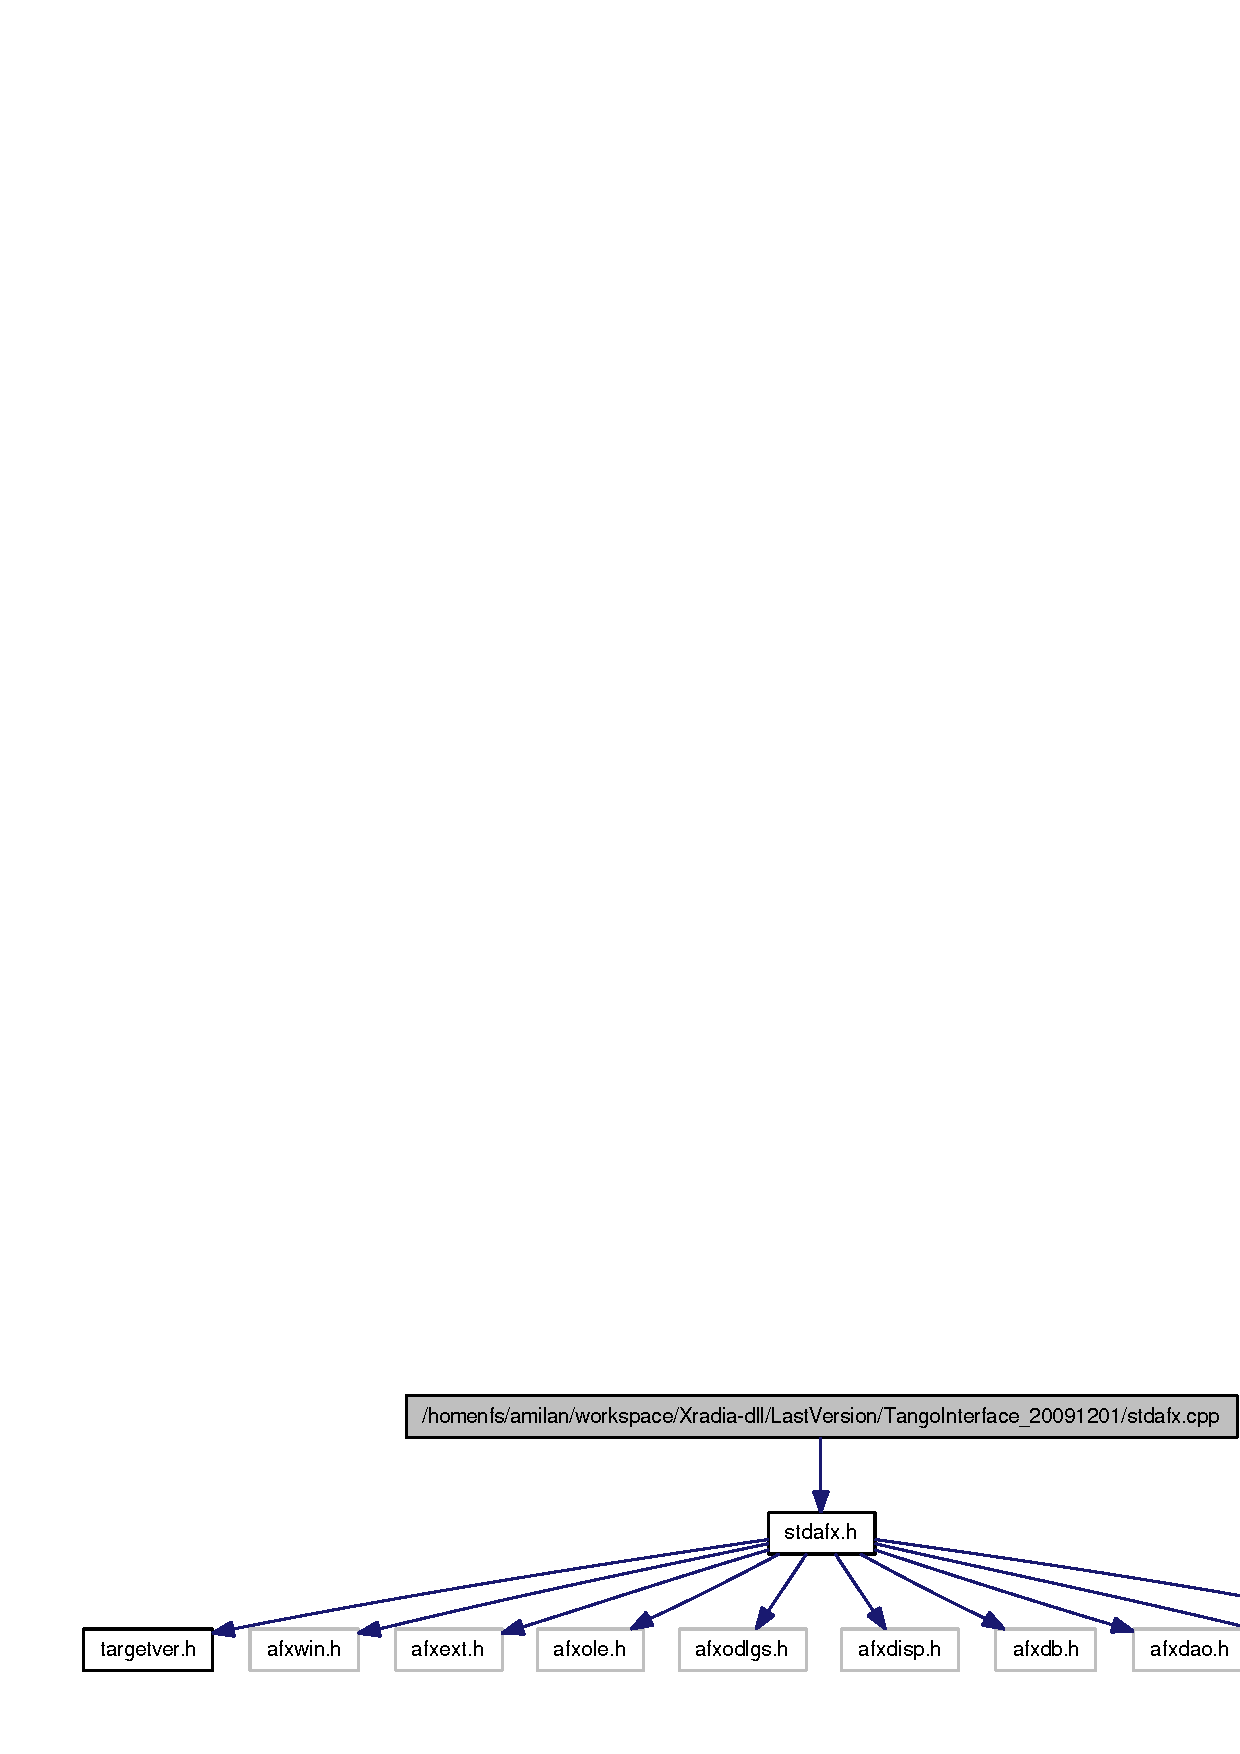
\includegraphics[width=375pt]{stdafx_8cpp__incl}
\end{center}
\end{figure}

\hypertarget{stdafx_8h}{
\section{/homenfs/amilan/workspace/Xradia-dll/LastVersion/TangoInterface\_\-20091201/stdafx.h File Reference}
\label{stdafx_8h}\index{/homenfs/amilan/workspace/Xradia-dll/LastVersion/TangoInterface\_\-20091201/stdafx.h@{/homenfs/amilan/workspace/Xradia-dll/LastVersion/TangoInterface\_\-20091201/stdafx.h}}
}
{\tt \#include \char`\"{}targetver.h\char`\"{}}\par
{\tt \#include $<$afxwin.h$>$}\par
{\tt \#include $<$afxext.h$>$}\par
{\tt \#include $<$afxole.h$>$}\par
{\tt \#include $<$afxodlgs.h$>$}\par
{\tt \#include $<$afxdisp.h$>$}\par
{\tt \#include $<$afxdb.h$>$}\par
{\tt \#include $<$afxdao.h$>$}\par
{\tt \#include $<$afxdtctl.h$>$}\par
{\tt \#include $<$afxcmn.h$>$}\par


Include dependency graph for stdafx.h:\nopagebreak
\begin{figure}[H]
\begin{center}
\leavevmode
\includegraphics[width=375pt]{stdafx_8h__incl}
\end{center}
\end{figure}


This graph shows which files directly or indirectly include this file:\nopagebreak
\begin{figure}[H]
\begin{center}
\leavevmode
\includegraphics[width=420pt]{stdafx_8h__dep__incl}
\end{center}
\end{figure}
\subsection*{Defines}
\begin{CompactItemize}
\item 
\#define \hyperlink{stdafx_8h_0172fbace36625330d5f0f163a1ddc1a}{VC\_\-EXTRALEAN}
\item 
\#define \hyperlink{stdafx_8h_137e19a46f145129447af81af06def9f}{\_\-ATL\_\-CSTRING\_\-EXPLICIT\_\-CONSTRUCTORS}
\end{CompactItemize}


\subsection{Define Documentation}
\hypertarget{stdafx_8h_137e19a46f145129447af81af06def9f}{
\index{stdafx.h@{stdafx.h}!\_\-ATL\_\-CSTRING\_\-EXPLICIT\_\-CONSTRUCTORS@{\_\-ATL\_\-CSTRING\_\-EXPLICIT\_\-CONSTRUCTORS}}
\index{\_\-ATL\_\-CSTRING\_\-EXPLICIT\_\-CONSTRUCTORS@{\_\-ATL\_\-CSTRING\_\-EXPLICIT\_\-CONSTRUCTORS}!stdafx.h@{stdafx.h}}
\subsubsection[\_\-ATL\_\-CSTRING\_\-EXPLICIT\_\-CONSTRUCTORS]{\setlength{\rightskip}{0pt plus 5cm}\#define \_\-ATL\_\-CSTRING\_\-EXPLICIT\_\-CONSTRUCTORS}}
\label{stdafx_8h_137e19a46f145129447af81af06def9f}


\hypertarget{stdafx_8h_0172fbace36625330d5f0f163a1ddc1a}{
\index{stdafx.h@{stdafx.h}!VC\_\-EXTRALEAN@{VC\_\-EXTRALEAN}}
\index{VC\_\-EXTRALEAN@{VC\_\-EXTRALEAN}!stdafx.h@{stdafx.h}}
\subsubsection[VC\_\-EXTRALEAN]{\setlength{\rightskip}{0pt plus 5cm}\#define VC\_\-EXTRALEAN}}
\label{stdafx_8h_0172fbace36625330d5f0f163a1ddc1a}



\hypertarget{TangoInterface_8cpp}{
\section{/homenfs/amilan/workspace/Xradia-dll/LastVersion/TangoInterface\_\-20091201/TangoInterface.cpp File Reference}
\label{TangoInterface_8cpp}\index{/homenfs/amilan/workspace/Xradia-dll/LastVersion/TangoInterface\_\-20091201/TangoInterface.cpp@{/homenfs/amilan/workspace/Xradia-dll/LastVersion/TangoInterface\_\-20091201/TangoInterface.cpp}}
}
{\tt \#include \char`\"{}stdafx.h\char`\"{}}\par
{\tt \#include \char`\"{}TangoInterface.h\char`\"{}}\par


Include dependency graph for TangoInterface.cpp:\nopagebreak
\begin{figure}[H]
\begin{center}
\leavevmode
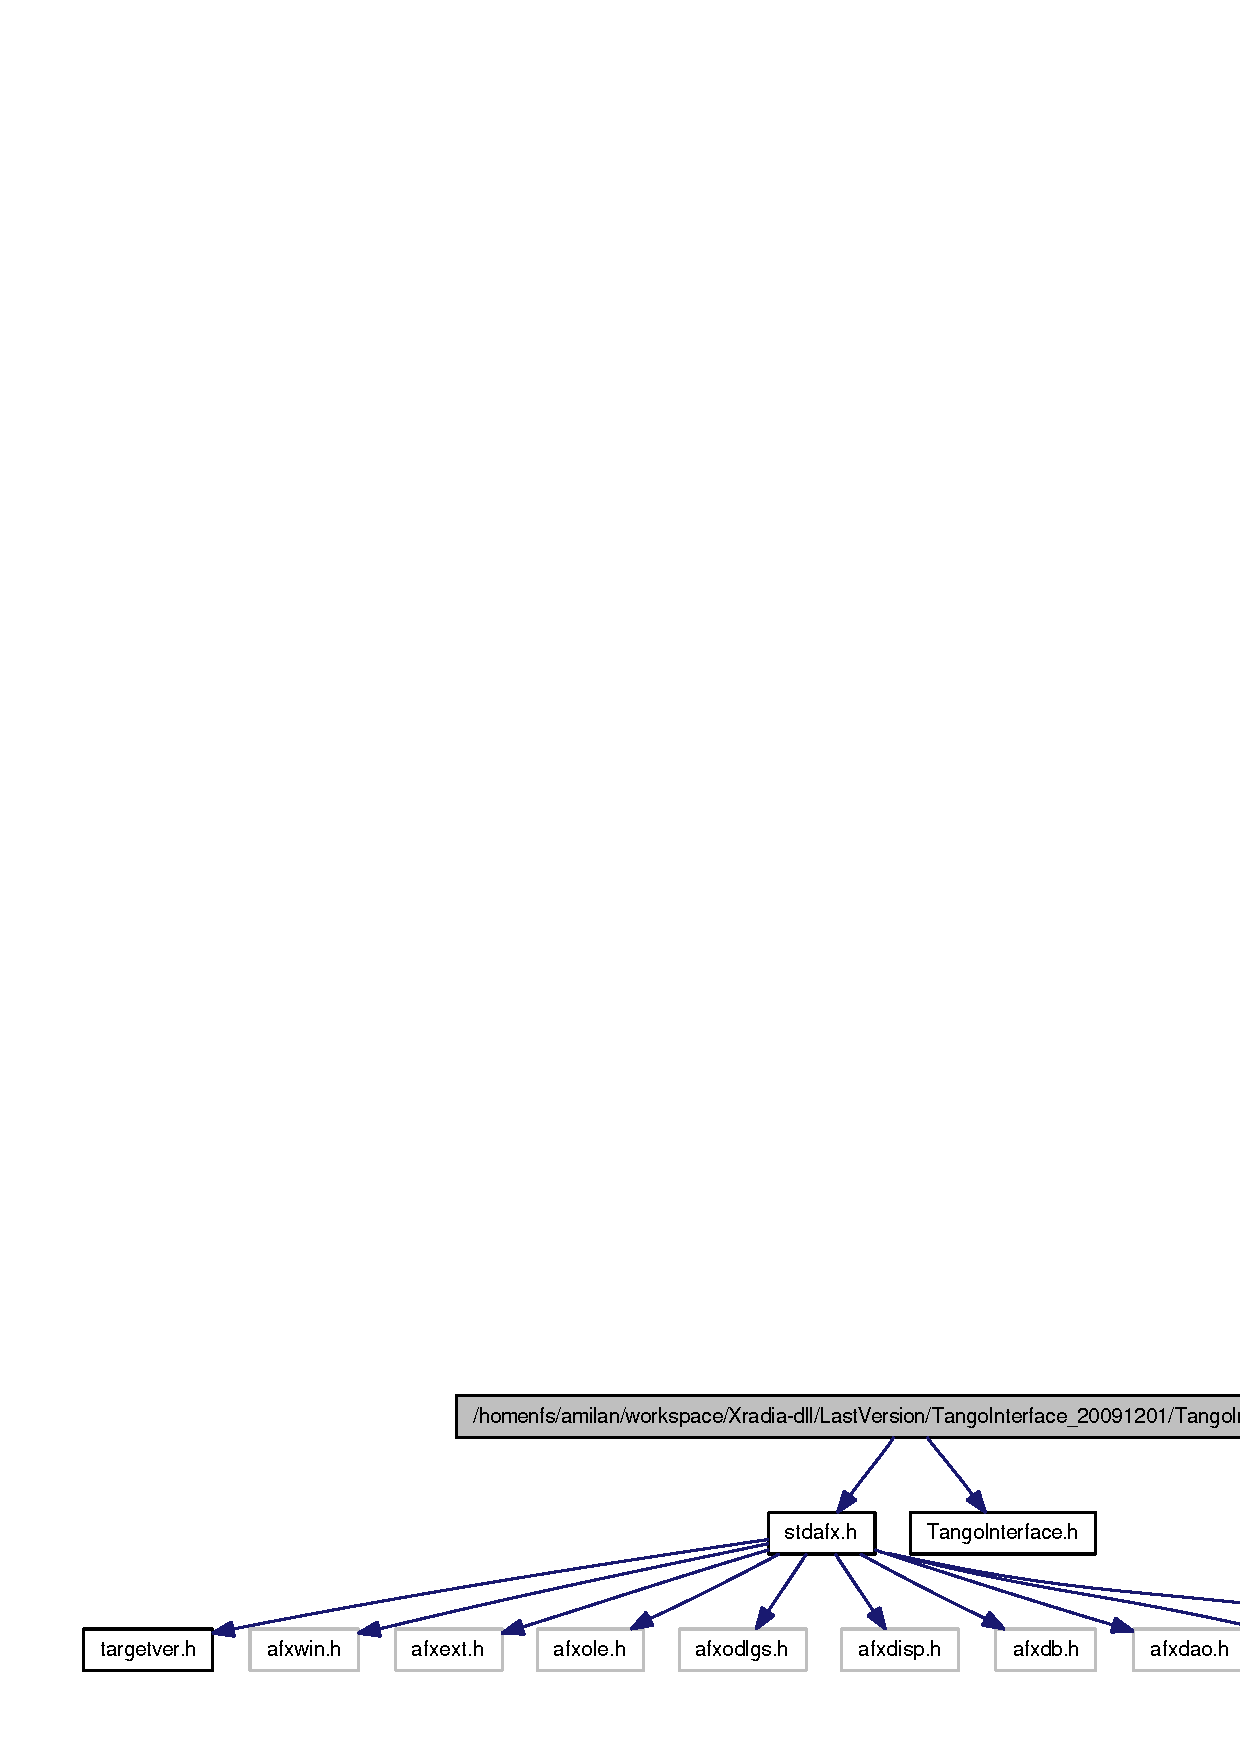
\includegraphics[width=375pt]{TangoInterface_8cpp__incl}
\end{center}
\end{figure}
\subsection*{Defines}
\begin{CompactItemize}
\item 
\#define \hyperlink{TangoInterface_8cpp_9c6419e7f541d4daf14f5ccd56e03f17}{NUM\_\-STRINGS}~7
\end{CompactItemize}


\subsection{Define Documentation}
\hypertarget{TangoInterface_8cpp_9c6419e7f541d4daf14f5ccd56e03f17}{
\index{TangoInterface.cpp@{TangoInterface.cpp}!NUM\_\-STRINGS@{NUM\_\-STRINGS}}
\index{NUM\_\-STRINGS@{NUM\_\-STRINGS}!TangoInterface.cpp@{TangoInterface.cpp}}
\subsubsection[NUM\_\-STRINGS]{\setlength{\rightskip}{0pt plus 5cm}\#define NUM\_\-STRINGS~7}}
\label{TangoInterface_8cpp_9c6419e7f541d4daf14f5ccd56e03f17}



\hypertarget{TangoInterface_8h}{
\section{/homenfs/amilan/workspace/Xradia-dll/LastVersion/TangoInterface\_\-20091201/TangoInterface.h File Reference}
\label{TangoInterface_8h}\index{/homenfs/amilan/workspace/Xradia-dll/LastVersion/TangoInterface\_\-20091201/TangoInterface.h@{/homenfs/amilan/workspace/Xradia-dll/LastVersion/TangoInterface\_\-20091201/TangoInterface.h}}
}


This graph shows which files directly or indirectly include this file:\nopagebreak
\begin{figure}[H]
\begin{center}
\leavevmode
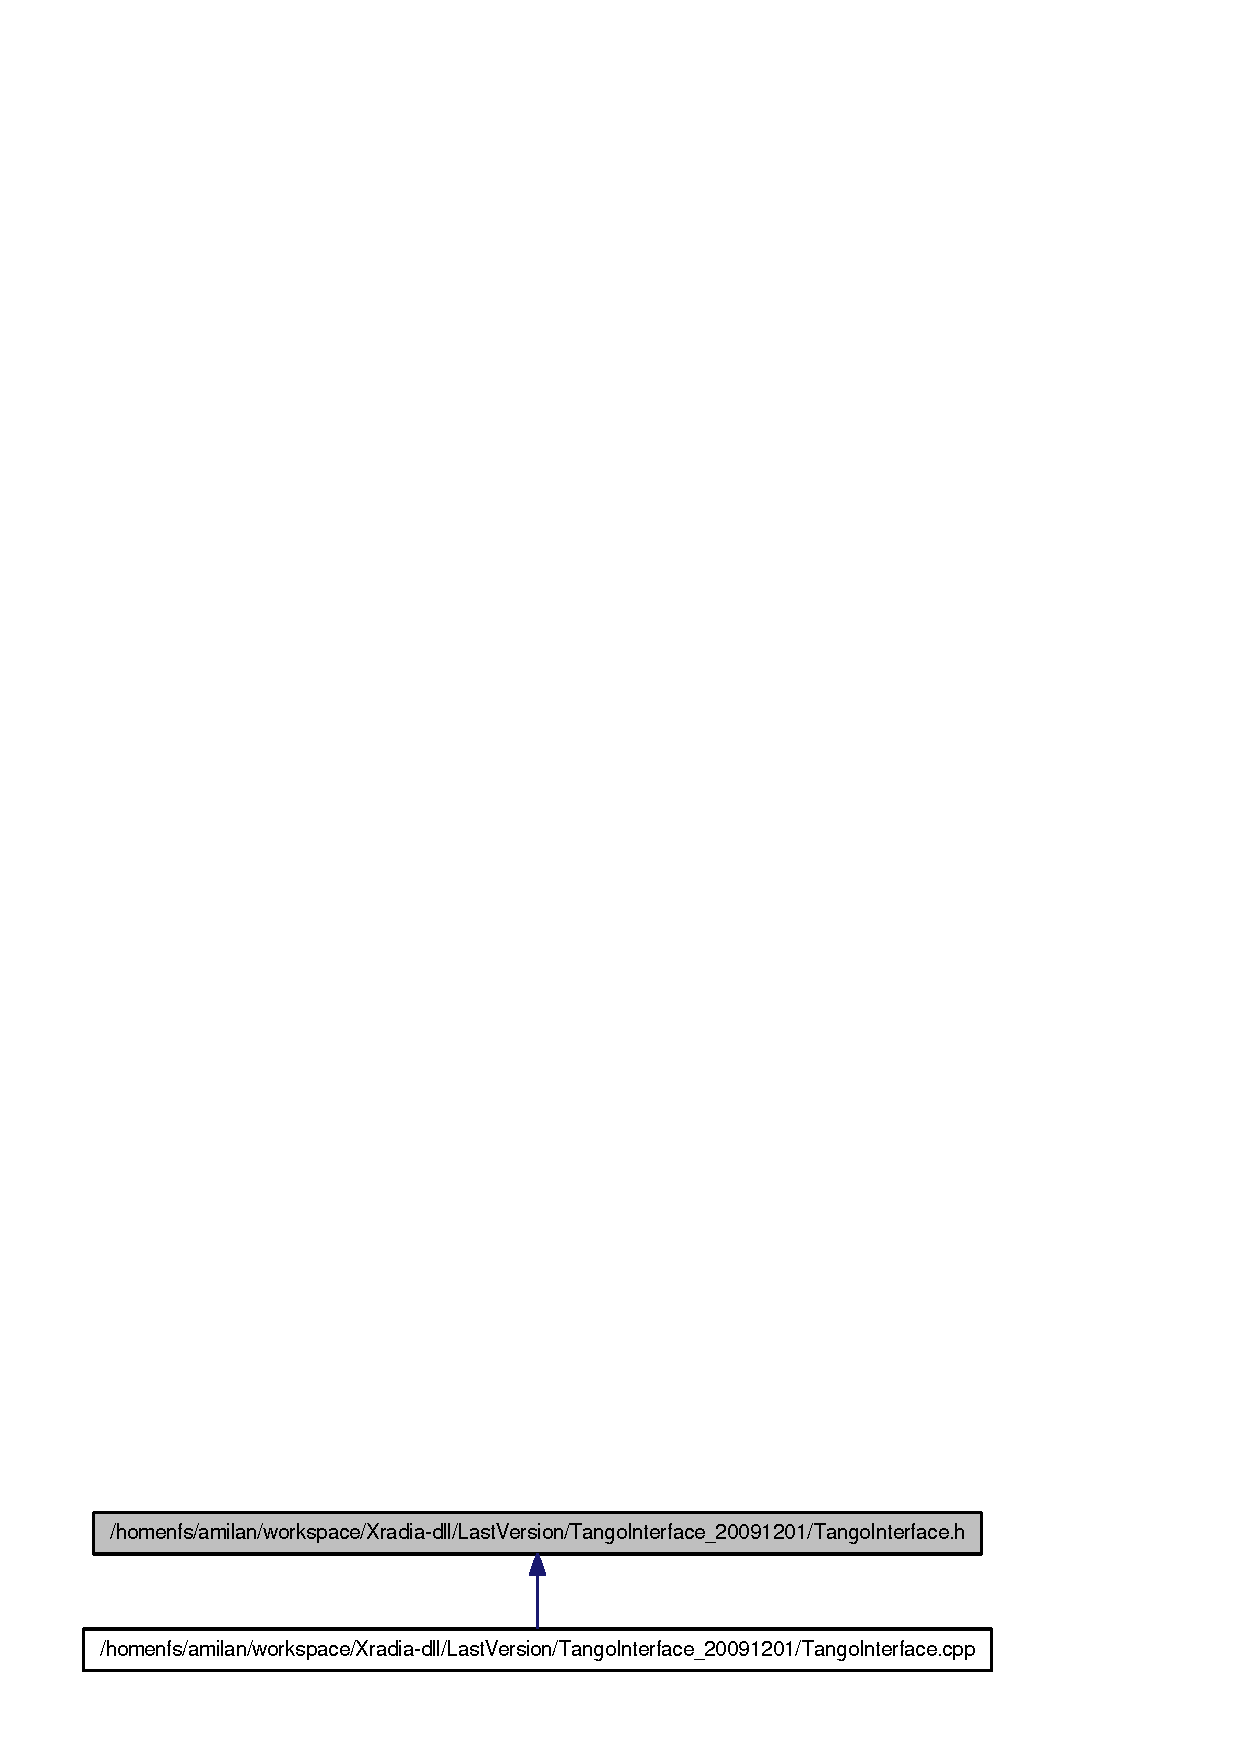
\includegraphics[width=240pt]{TangoInterface_8h__dep__incl}
\end{center}
\end{figure}
\subsection*{Classes}
\begin{CompactItemize}
\item 
class \hyperlink{classTangoInterface}{TangoInterface}
\end{CompactItemize}
\subsection*{Enumerations}
\begin{CompactItemize}
\item 
enum \hyperlink{TangoInterface_8h_76084dde89360059bf6c314f19df5895}{TANGO\_\-ATTRIBUTES} \{ \par
\hyperlink{TangoInterface_8h_76084dde89360059bf6c314f19df58952bfb5bacab2fb8adac5fea24deb94fef}{NEG\_\-LIMIT} =  0, 
\hyperlink{TangoInterface_8h_76084dde89360059bf6c314f19df5895e5680034e53fb79da9445a56b52774ed}{POS\_\-LIMIT}, 
\hyperlink{TangoInterface_8h_76084dde89360059bf6c314f19df58953a32f93ff061954504e42fc5cfcb1d52}{IN\_\-POS}, 
\hyperlink{TangoInterface_8h_76084dde89360059bf6c314f19df5895d853c51c0c284231f7a3b7640763f058}{FOLLOWING\_\-ERROR}, 
\par
\hyperlink{TangoInterface_8h_76084dde89360059bf6c314f19df589599788d1f27bac42d0c7bac63026c5959}{ENABLED}, 
\hyperlink{TangoInterface_8h_76084dde89360059bf6c314f19df5895b8a476105cd4aa2b5dbb6223bad8878b}{MOTOR\_\-POSITION}, 
\hyperlink{TangoInterface_8h_76084dde89360059bf6c314f19df5895a1633da4d7554a30c3f0ba1a62c1284e}{SET\_\-VELO}, 
\hyperlink{TangoInterface_8h_76084dde89360059bf6c314f19df589598914338f9b2ae18755a393bfccce8cb}{CURRENT\_\-SIZE\_\-TANGO\_\-ATTRIBUTES\_\-ENUM}
 \}
\begin{CompactList}\small\item\em Tango interface. \item\end{CompactList}\end{CompactItemize}


\subsection{Enumeration Type Documentation}
\hypertarget{TangoInterface_8h_76084dde89360059bf6c314f19df5895}{
\index{TangoInterface.h@{TangoInterface.h}!TANGO\_\-ATTRIBUTES@{TANGO\_\-ATTRIBUTES}}
\index{TANGO\_\-ATTRIBUTES@{TANGO\_\-ATTRIBUTES}!TangoInterface.h@{TangoInterface.h}}
\subsubsection[TANGO\_\-ATTRIBUTES]{\setlength{\rightskip}{0pt plus 5cm}enum {\bf TANGO\_\-ATTRIBUTES}}}
\label{TangoInterface_8h_76084dde89360059bf6c314f19df5895}


Tango interface. 

One object will be used for contacting all Tango axes. The primary design of this class is to communicate with Tango motors. It also has the facility to communicate with any Tango variable for recording external data.

Units: Assumed in all functions that the units of the passed in values are the same. Xradia software will have a conversion factor that will allow the Xradia software to use Engineering units (ex. mm, deg, eV) independent of the actual hardware. In all descriptions below, the units will be referred to generically as \char`\"{}counts\char`\"{}.

Motor Identifier: The motor identifier is a freeform string (configured per motor) that contains all information necessary to connect to a particular hosted motor. The definition of this string is left to the implementor of this interface. \begin{Desc}
\item[Enumerator: ]\par
\begin{description}
\index{NEG\_\-LIMIT@{NEG\_\-LIMIT}!TangoInterface.h@{TangoInterface.h}}\index{TangoInterface.h@{TangoInterface.h}!NEG\_\-LIMIT@{NEG\_\-LIMIT}}\item[{\em 
\hypertarget{TangoInterface_8h_76084dde89360059bf6c314f19df58952bfb5bacab2fb8adac5fea24deb94fef}{
NEG\_\-LIMIT}
\label{TangoInterface_8h_76084dde89360059bf6c314f19df58952bfb5bacab2fb8adac5fea24deb94fef}
}]\index{POS\_\-LIMIT@{POS\_\-LIMIT}!TangoInterface.h@{TangoInterface.h}}\index{TangoInterface.h@{TangoInterface.h}!POS\_\-LIMIT@{POS\_\-LIMIT}}\item[{\em 
\hypertarget{TangoInterface_8h_76084dde89360059bf6c314f19df5895e5680034e53fb79da9445a56b52774ed}{
POS\_\-LIMIT}
\label{TangoInterface_8h_76084dde89360059bf6c314f19df5895e5680034e53fb79da9445a56b52774ed}
}]\index{IN\_\-POS@{IN\_\-POS}!TangoInterface.h@{TangoInterface.h}}\index{TangoInterface.h@{TangoInterface.h}!IN\_\-POS@{IN\_\-POS}}\item[{\em 
\hypertarget{TangoInterface_8h_76084dde89360059bf6c314f19df58953a32f93ff061954504e42fc5cfcb1d52}{
IN\_\-POS}
\label{TangoInterface_8h_76084dde89360059bf6c314f19df58953a32f93ff061954504e42fc5cfcb1d52}
}]\index{FOLLOWING\_\-ERROR@{FOLLOWING\_\-ERROR}!TangoInterface.h@{TangoInterface.h}}\index{TangoInterface.h@{TangoInterface.h}!FOLLOWING\_\-ERROR@{FOLLOWING\_\-ERROR}}\item[{\em 
\hypertarget{TangoInterface_8h_76084dde89360059bf6c314f19df5895d853c51c0c284231f7a3b7640763f058}{
FOLLOWING\_\-ERROR}
\label{TangoInterface_8h_76084dde89360059bf6c314f19df5895d853c51c0c284231f7a3b7640763f058}
}]\index{ENABLED@{ENABLED}!TangoInterface.h@{TangoInterface.h}}\index{TangoInterface.h@{TangoInterface.h}!ENABLED@{ENABLED}}\item[{\em 
\hypertarget{TangoInterface_8h_76084dde89360059bf6c314f19df589599788d1f27bac42d0c7bac63026c5959}{
ENABLED}
\label{TangoInterface_8h_76084dde89360059bf6c314f19df589599788d1f27bac42d0c7bac63026c5959}
}]\index{MOTOR\_\-POSITION@{MOTOR\_\-POSITION}!TangoInterface.h@{TangoInterface.h}}\index{TangoInterface.h@{TangoInterface.h}!MOTOR\_\-POSITION@{MOTOR\_\-POSITION}}\item[{\em 
\hypertarget{TangoInterface_8h_76084dde89360059bf6c314f19df5895b8a476105cd4aa2b5dbb6223bad8878b}{
MOTOR\_\-POSITION}
\label{TangoInterface_8h_76084dde89360059bf6c314f19df5895b8a476105cd4aa2b5dbb6223bad8878b}
}]\index{SET\_\-VELO@{SET\_\-VELO}!TangoInterface.h@{TangoInterface.h}}\index{TangoInterface.h@{TangoInterface.h}!SET\_\-VELO@{SET\_\-VELO}}\item[{\em 
\hypertarget{TangoInterface_8h_76084dde89360059bf6c314f19df5895a1633da4d7554a30c3f0ba1a62c1284e}{
SET\_\-VELO}
\label{TangoInterface_8h_76084dde89360059bf6c314f19df5895a1633da4d7554a30c3f0ba1a62c1284e}
}]\index{CURRENT\_\-SIZE\_\-TANGO\_\-ATTRIBUTES\_\-ENUM@{CURRENT\_\-SIZE\_\-TANGO\_\-ATTRIBUTES\_\-ENUM}!TangoInterface.h@{TangoInterface.h}}\index{TangoInterface.h@{TangoInterface.h}!CURRENT\_\-SIZE\_\-TANGO\_\-ATTRIBUTES\_\-ENUM@{CURRENT\_\-SIZE\_\-TANGO\_\-ATTRIBUTES\_\-ENUM}}\item[{\em 
\hypertarget{TangoInterface_8h_76084dde89360059bf6c314f19df589598914338f9b2ae18755a393bfccce8cb}{
CURRENT\_\-SIZE\_\-TANGO\_\-ATTRIBUTES\_\-ENUM}
\label{TangoInterface_8h_76084dde89360059bf6c314f19df589598914338f9b2ae18755a393bfccce8cb}
}]\end{description}
\end{Desc}


\hypertarget{TangoInterfaceApp_8cpp}{
\section{/homenfs/amilan/workspace/Xradia-dll/LastVersion/TangoInterface\_\-20091201/TangoInterfaceApp.cpp File Reference}
\label{TangoInterfaceApp_8cpp}\index{/homenfs/amilan/workspace/Xradia-dll/LastVersion/TangoInterface\_\-20091201/TangoInterfaceApp.cpp@{/homenfs/amilan/workspace/Xradia-dll/LastVersion/TangoInterface\_\-20091201/TangoInterfaceApp.cpp}}
}
{\tt \#include \char`\"{}stdafx.h\char`\"{}}\par
{\tt \#include \char`\"{}TangoInterfaceApp.h\char`\"{}}\par


Include dependency graph for TangoInterfaceApp.cpp:\nopagebreak
\begin{figure}[H]
\begin{center}
\leavevmode
\includegraphics[width=415pt]{TangoInterfaceApp_8cpp__incl}
\end{center}
\end{figure}
\subsection*{Variables}
\begin{CompactItemize}
\item 
\hyperlink{classCTangoInterfaceApp}{CTangoInterfaceApp} \hyperlink{TangoInterfaceApp_8cpp_9e57ea710d0558dda8961bdb57cd3bc9}{theApp}
\end{CompactItemize}


\subsection{Variable Documentation}
\hypertarget{TangoInterfaceApp_8cpp_9e57ea710d0558dda8961bdb57cd3bc9}{
\index{TangoInterfaceApp.cpp@{TangoInterfaceApp.cpp}!theApp@{theApp}}
\index{theApp@{theApp}!TangoInterfaceApp.cpp@{TangoInterfaceApp.cpp}}
\subsubsection[theApp]{\setlength{\rightskip}{0pt plus 5cm}{\bf CTangoInterfaceApp} {\bf theApp}}}
\label{TangoInterfaceApp_8cpp_9e57ea710d0558dda8961bdb57cd3bc9}



\hypertarget{TangoInterfaceApp_8h}{
\section{/homenfs/amilan/workspace/Xradia-dll/LastVersion/TangoInterface\_\-20091201/TangoInterfaceApp.h File Reference}
\label{TangoInterfaceApp_8h}\index{/homenfs/amilan/workspace/Xradia-dll/LastVersion/TangoInterface\_\-20091201/TangoInterfaceApp.h@{/homenfs/amilan/workspace/Xradia-dll/LastVersion/TangoInterface\_\-20091201/TangoInterfaceApp.h}}
}
{\tt \#include \char`\"{}resource.h\char`\"{}}\par


Include dependency graph for TangoInterfaceApp.h:\nopagebreak
\begin{figure}[H]
\begin{center}
\leavevmode
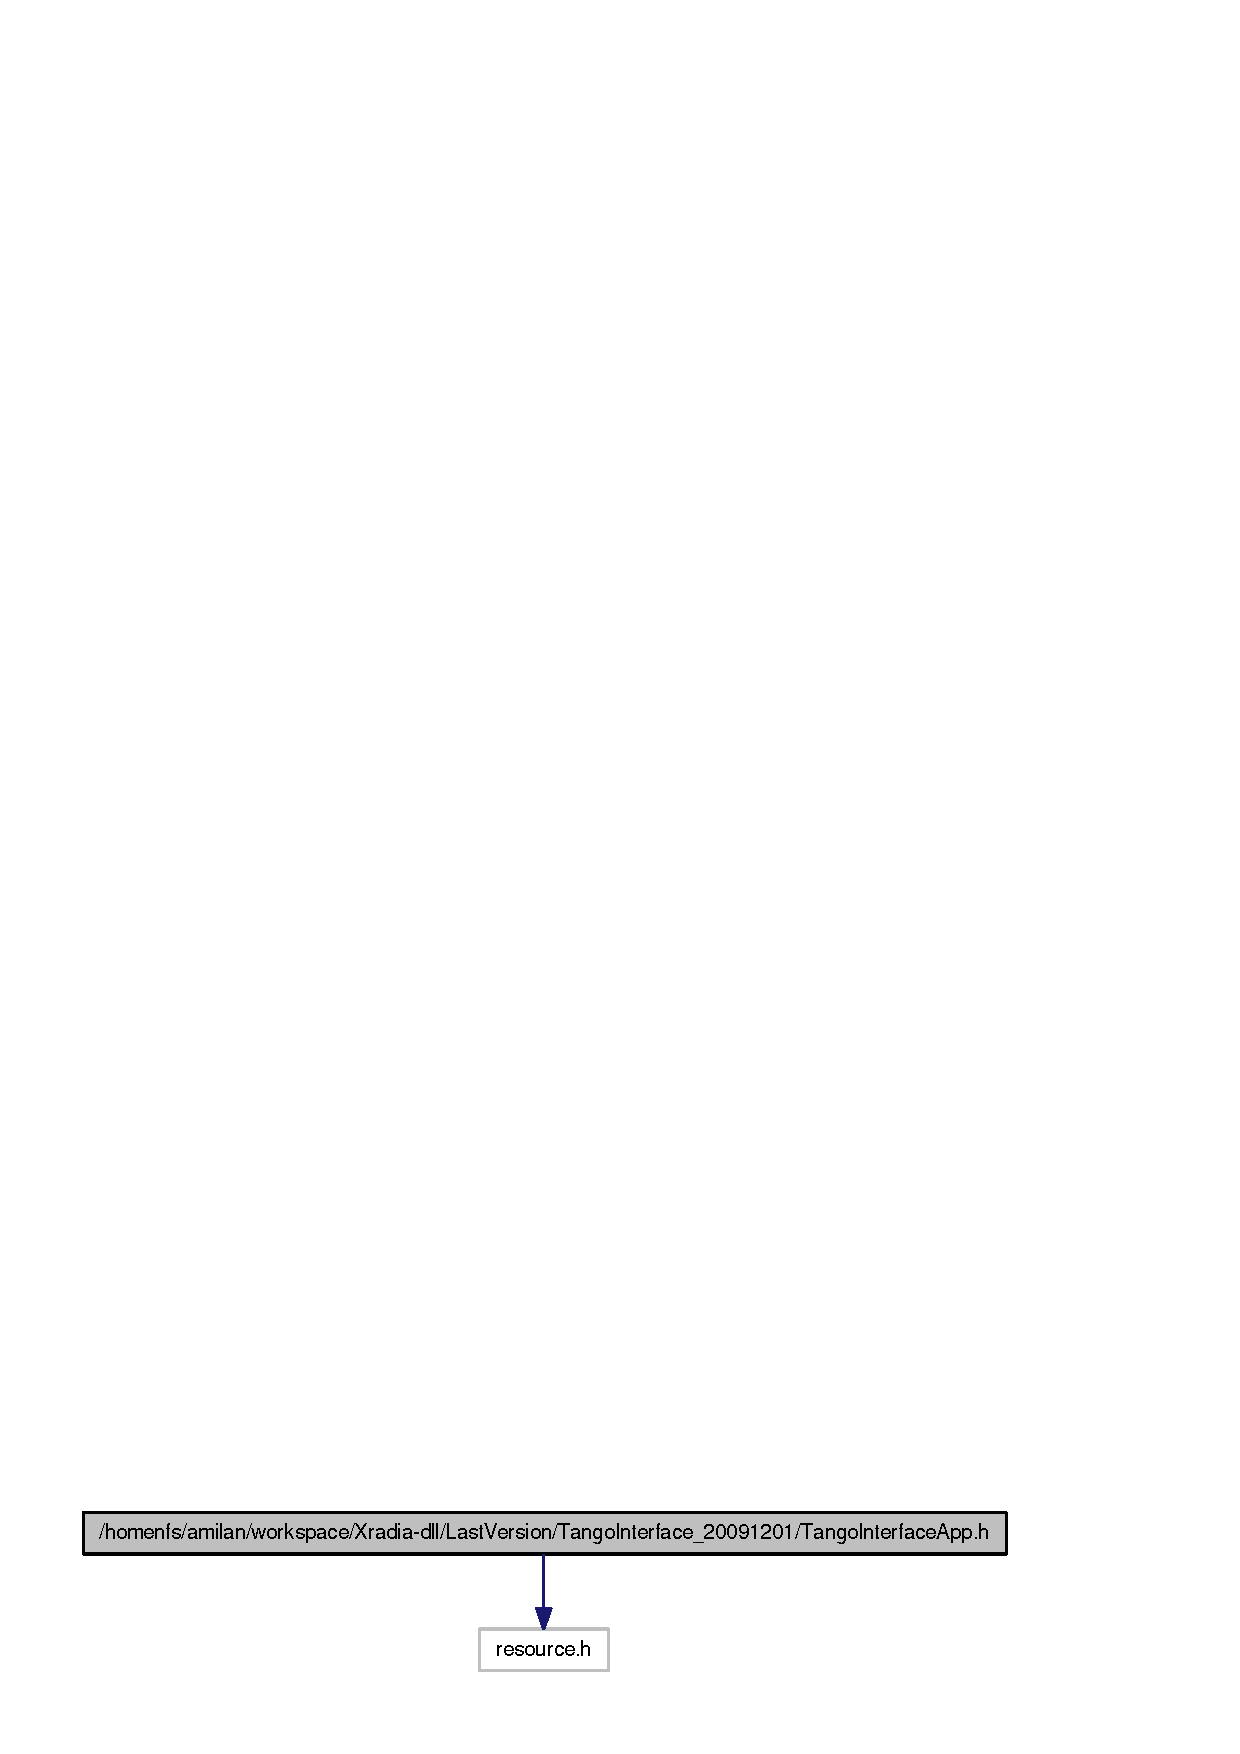
\includegraphics[width=243pt]{TangoInterfaceApp_8h__incl}
\end{center}
\end{figure}


This graph shows which files directly or indirectly include this file:\nopagebreak
\begin{figure}[H]
\begin{center}
\leavevmode
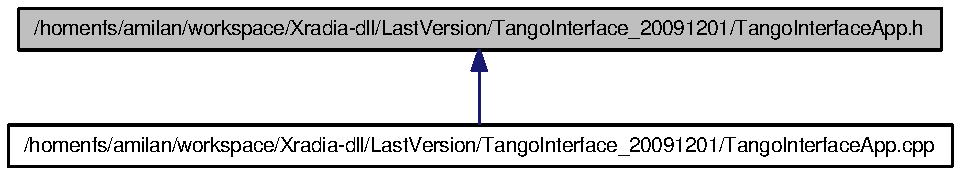
\includegraphics[width=248pt]{TangoInterfaceApp_8h__dep__incl}
\end{center}
\end{figure}
\subsection*{Classes}
\begin{CompactItemize}
\item 
class \hyperlink{classCTangoInterfaceApp}{CTangoInterfaceApp}
\end{CompactItemize}

\hypertarget{targetver_8h}{
\section{/homenfs/amilan/workspace/Xradia-dll/LastVersion/TangoInterface\_\-20091201/targetver.h File Reference}
\label{targetver_8h}\index{/homenfs/amilan/workspace/Xradia-dll/LastVersion/TangoInterface\_\-20091201/targetver.h@{/homenfs/amilan/workspace/Xradia-dll/LastVersion/TangoInterface\_\-20091201/targetver.h}}
}


This graph shows which files directly or indirectly include this file:\nopagebreak
\begin{figure}[H]
\begin{center}
\leavevmode
\includegraphics[width=420pt]{targetver_8h__dep__incl}
\end{center}
\end{figure}
\subsection*{Defines}
\begin{CompactItemize}
\item 
\#define \hyperlink{targetver_8h_966cd377b9f3fdeb1432460c33352af1}{WINVER}~0x0502
\item 
\#define \hyperlink{targetver_8h_c50762666aa00bd3a4308158510f1748}{\_\-WIN32\_\-WINNT}~0x0502
\item 
\#define \hyperlink{targetver_8h_074ca98c073d899c62fc6629918186c8}{\_\-WIN32\_\-WINDOWS}~0x0410
\item 
\#define \hyperlink{targetver_8h_d4562ce705fe4682e63dc8f1ea9dd344}{\_\-WIN32\_\-IE}~0x0700
\end{CompactItemize}


\subsection{Define Documentation}
\hypertarget{targetver_8h_d4562ce705fe4682e63dc8f1ea9dd344}{
\index{targetver.h@{targetver.h}!\_\-WIN32\_\-IE@{\_\-WIN32\_\-IE}}
\index{\_\-WIN32\_\-IE@{\_\-WIN32\_\-IE}!targetver.h@{targetver.h}}
\subsubsection[\_\-WIN32\_\-IE]{\setlength{\rightskip}{0pt plus 5cm}\#define \_\-WIN32\_\-IE~0x0700}}
\label{targetver_8h_d4562ce705fe4682e63dc8f1ea9dd344}


\hypertarget{targetver_8h_074ca98c073d899c62fc6629918186c8}{
\index{targetver.h@{targetver.h}!\_\-WIN32\_\-WINDOWS@{\_\-WIN32\_\-WINDOWS}}
\index{\_\-WIN32\_\-WINDOWS@{\_\-WIN32\_\-WINDOWS}!targetver.h@{targetver.h}}
\subsubsection[\_\-WIN32\_\-WINDOWS]{\setlength{\rightskip}{0pt plus 5cm}\#define \_\-WIN32\_\-WINDOWS~0x0410}}
\label{targetver_8h_074ca98c073d899c62fc6629918186c8}


\hypertarget{targetver_8h_c50762666aa00bd3a4308158510f1748}{
\index{targetver.h@{targetver.h}!\_\-WIN32\_\-WINNT@{\_\-WIN32\_\-WINNT}}
\index{\_\-WIN32\_\-WINNT@{\_\-WIN32\_\-WINNT}!targetver.h@{targetver.h}}
\subsubsection[\_\-WIN32\_\-WINNT]{\setlength{\rightskip}{0pt plus 5cm}\#define \_\-WIN32\_\-WINNT~0x0502}}
\label{targetver_8h_c50762666aa00bd3a4308158510f1748}


\hypertarget{targetver_8h_966cd377b9f3fdeb1432460c33352af1}{
\index{targetver.h@{targetver.h}!WINVER@{WINVER}}
\index{WINVER@{WINVER}!targetver.h@{targetver.h}}
\subsubsection[WINVER]{\setlength{\rightskip}{0pt plus 5cm}\#define WINVER~0x0502}}
\label{targetver_8h_966cd377b9f3fdeb1432460c33352af1}



\printindex
\end{document}
